
\chapter{Conclusion}
\label{cpt:conclusion}

\section{Conclusion}

\begin{figure}[ht]
    \centering
    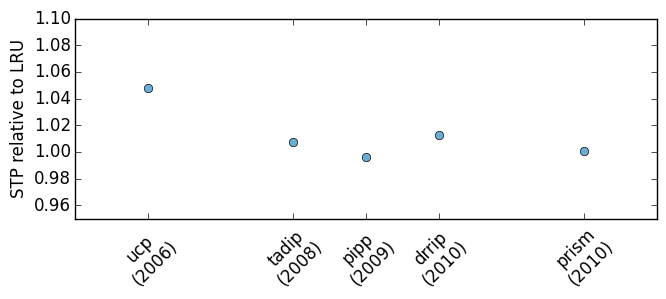
\includegraphics[width=\textwidth]{figures/results/speedup/year-comp}
    \caption[Average algorithm performance by year of publication]{Average algorithm performance measured in STP and HMS normalized to \gls{lru} by year of publication.}
    \label{fig:conclusion:yearcomp}
\end{figure}

In this thesis, we have curated a list of important and recent work in the cache management research field.
We have presented a theoretical explanation of all algorithms and compared them with each other.
A simulation framework based on Sniper was created, and several of the algorithms presented have been implemented within this framework.
We have presented some potential error sources within Sniper; most notably is the lack of precision when simulating inter-core interactions.
However, experiments were conducted to investigate the severity of this inaccuracy, and based on the results we conclude that Sniper is a viable choice for this research.

Figure~\ref{fig:conclusion:yearcomp} is a highly simplified view of our results, showing average STP and HMS for all algorithms by publication year, normalized to \gls{lru} performance.
Throughout our work, UCP has proven to be the best performer providing up to 5\% speedups measured in STP for our main experiment.
With constrained resources, we observed more than 20\% performance improvement with UCP.
PIPP has been unable to compete with \gls{lru} in most cases, and on average performed no better than \gls{lru}.
We suspect this is due to a short lifetime of cache blocks in a PIPP managed cache.
Both DRRIP and TADIP, which are arguably simpler schemes compared to UCP and PIPP, have shown to outperform \gls{lru}.
Neither has been able to achieve speedups comparable to UCP.
In terms of misses, we have observed that DRRIP, TADIP, and PriSM, which all attempt to reduce overall misses succeed by having as many or fewer misses than \gls{lru}.
UCP has proven to cause an increased number of misses.
We suspect that this may be an artifact of the greedy lookahead algorithm, which prioritizes high marginal utility and that might not always equal fewer misses.
Section~\ref{sec:results:cache_partition} covers in detail how this might result in both increased miss count and performance in the same workload.


Independent of the performance metric used, none of the implemented algorithms has proven to beat UCP on average.
Our results make it is tempting to conclude that UCP is the best solution.
In sections~\ref{sec:results:l3size_sensitivity} and~\ref{sec:results:bus_sensitivity} we demonstrated that changes in the simulated architecture can greatly affect algorithm performance, and in all cases UCP had a positive trend.
While we claim that UCP is the best solution in our setup, this might not be the case in all architectural configurations.
\gls{lru} is still the dominating algorithm in hardware implementations, even if UCP has existed for nine years, and several publications have shown its improvement over \gls{lru}.
Compared to \gls{lru}, UCP requires more hardware to implement. 
In a real design process, this additional hardware will come at the cost of reduced area for some other functionality.
In the end, this might cause the improvement of cache performance to be reverted by a decrease in performance of some other component.

\section{Future Work}

The time constraints put on this thesis has limited the number of algorithms presented.
Given more time we would like to continue exploring the vast research field that is cache management, and bring further algorithms into this comparison.
Implementing more algorithms within the simulation framework would also allow for more interesting results.

The Sniper simulation system has integrations to various power estimation tools.
Given that power is a concern when designing processor cores today, it would make sense to extend the simulation framework to provide power estimations as well.
With this data at hand, we would be able to use not only performance but also increased power consumption when comparing algorithms.
The potential for implementing this was not considered during this thesis, mainly because of the time constraint.

\section{Acknowledgement}
The author would like to thank Associate Professor Magnus
Jahre and \todo{Title?} Researcher Antonio Garcia Guirado at the Department of Computer and Information Science, Norwegian University of Science and Technology, for their excellent guidance and useful critique during the planning and realization of this thesis.
The author would also like to thank his fiancée and family for all their support and encouragement throughout his studies.
All of our experiments were run on the Stallo cluster under Nortur grant nn4650k.